\documentclass{article}

% Language setting
% Replace `english' with e.g. `spanish' to change the document language
\usepackage[english]{babel}
\usepackage{multicol}
\usepackage{float}

% Set page size and margins
% Replace `letterpaper' with`a4paper' for UK/EU standard size
\usepackage[letterpaper,top=2cm,bottom=2cm,left=3cm,right=3cm,marginparwidth=1.75cm]{geometry}

% Useful packages
\usepackage{amsmath}
\usepackage{graphicx}
\usepackage[colorlinks=true, allcolors=blue]{hyperref}

\title{Implementing the SIFT algorithm}
\author{Huy Nguyen (40090345)\\
GitHub: https://github.com/giahuy22012000/ImplementingSIFT
}

\begin{document}
\maketitle

\begin{multicols}{2}
	
	\begin{abstract}
		In this project, we attempt to implement our version of the SIFT algorithm invented by David Lowe.
	\end{abstract}
	
	\section{Background}
	Feature Description along with other techniques such as corner and shape detection formed the main foundation for semantic image processing until the dawn of deep learning and other neural network based approaches.
	
	Scale-Invariant Feature Transform or SIFT was invented by David Lowe in 1999, as a computer vision algorithm to detect and describe features in images \cite{wiki}. SIFT is well known for its ability to detect features across different scale levels and its robustness against change in contrast, orientation and lumination. Therefore, SIFT algorithm has a wide range of applications such as image stitching, object tracking, and terrain mapping.
	In this project, we attempt to implement our version of the algorithm as described in Lowe's paper \cite{Lowe:2004:DIF:993451.996342}.
	
	
	\section{Implementation}
	The implementation of the said algorithm is done in successive states where the the result of one function call is passed to the next one.
	
	\subsection{Scale-space Extrema Detection}
	Features are defined as patches of an image that contain a relatively unique arrangement and fluctuation in pixel values to make it easily identifiable against the rest of the image. There are serveral approach to locate these keypoints. One of such methods is Harris Corner algorithm which is based on our percention and tendency to inherently look for corners when presented with an image. The method works well at locating corners through computing and evaluating the "corness" value for each keypoint from image gradients. However, the draw back of Harris Corner approach is that its result usually is sensitive to image scale \ref{fig:sift_scale_invariant}. 
	
	\begin{figure*}
		\centering
		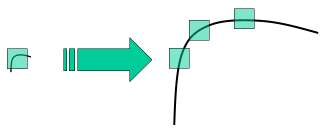
\includegraphics[width=0.4\linewidth]{sift_scale_invariant.jpg}
		\caption{\label{fig:sift_scale_invariant} Harris corner scale variant}
	\end{figure*}
	
	SIFT algorithm addresses the scale variant issue by searching for keypoints not only on the original 1x scale of the image but also its downsampled versions. The algorithm takes advantage of the nature of Laplacian of Gaussian (LoG) filter to bring out non uniform regions of an image thus significantly reduces that search space for keypoints. Although this seems to be archieving the same result as corner searching using Harris Corner algorithm, SIFT keypoint search is often practically faster since it uses Difference of Gaussian (DoG) to approximate Laplacian of Gaussian which is more computationally expensive. In fact, for each scale of an image, SIFT algorithm applies Gaussian filters with sigma values varied by a factor ($K=\sqrt{2}$ is used in the project) to get images of different blur levels. This process is then repeated for the half downsampled version of the previous. Each of the sets of blured images on a same scale is called an octave \cite{Lowe:2004:DIF:993451.996342}. Every two adjacent blured image in the same octave is substracted to get the Difference of Gaussian \ref*{sift_dog}. In the notebook, this process is done in $detectExtrema()$ function.
	
	\begin{figure*}
		\centering
		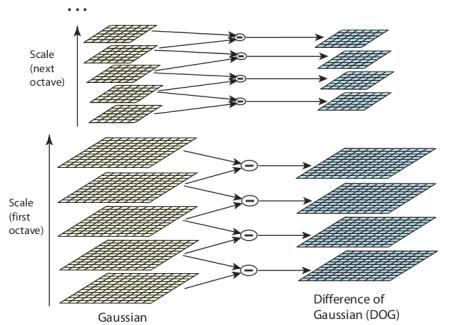
\includegraphics[width=0.4\linewidth]{sift_dog.jpg}
		\caption{\label{fig:sift_dog} SIFT's Difference of Gaussian}
	\end{figure*}
	
	As per the paper, keypoints are searched among three consecutive images with different sigma values (scales) \ref{sift_local_extrema}. The process is demonstrated in $locateKeypoints()$ function in the notebook which we go through images with different blur levels from the second to second last position in each octave and compare the center pixel to their 28 neighbors. The indices are interpolated back to the original image size and save both in binary map and a list of OpenCV built-in $Keypoint$ objects. The result from calling the function are then drawn on the original image using OpenCV $drawKeypoints()$ function \ref{locateKeypoints}.
	
	\begin{figure*}
		\centering
		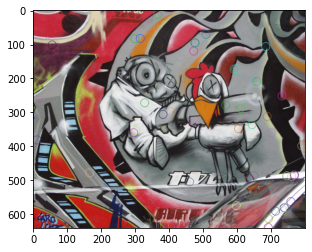
\includegraphics[width=0.4\linewidth]{locateKeypoints.png}
		\caption{\label{fig:locateKeypoints} Detected keypoints}
	\end{figure*}
	
	\subsection{Keypoint Localization}
	In this step, the keypoints are refined and thredhold so as to keep only a quality set using various techniques. However, since in this example, we have not yet to optimize the scale-space extrema extraction, only a small set of keypoints are obtained from previous step. As shown in the notebook, we skip the keypoint localization step.
	
	\subsection{Orientation Assignment}
	The basic idea behind this steps is for each keypoint, we assign it with a orientation ($0\deg to 360\deg$) obtained by looking at the keypoint's 4x4 neighborhood orientation histogram. The process is implemented in the notebook under $assignOrientation()$ function. By looping through the set of keypoints returned by previous steps, we extract the keypoint's neighborhood 4x4 window with index $[1,1]$ being the keypoint's location. A list of size 36 is created to accumulate the keypoint's gradient magnitude adjusted by a Gaussian convolution. By calculating the two gradient components at each pixel in the window, we can easily compute its gradient orientation and magnitude using the following fomulas.
	
	\begin{align*}
		\Theta       & =\arctan{\frac{\partial y}{\partial x}} 
		\| \nabla \| & =\sqrt{(\partial x)^2 + {\partial y}^2} 
	\end{align*}
	
	The orientations $\Theta$ are then categorized into their respective bins (in $10\deg$ increments) in the histogram. Using Numpy built-in $argmax()$ function, we can find the dominant orientation in the keypoint's neighborhood histogram and assign it to the keypoint. One of the histogram as demostrated in the notebook may look like this:
	
	\begin{figure*}
		\centering
		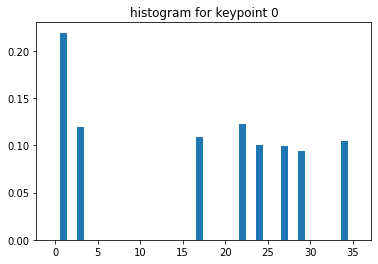
\includegraphics[width=0.4\linewidth]{36histogram.png}
		\caption{\label{fig:36histogram} A typical 36-bin orientation histogram}
	\end{figure*}	
	
	
	\subsection{Keypoint Descriptor}
	After being assigned an orientation, the keypoints go into a process to create a identifier vector called keypoint descriptions. In the notebook, it is implemented in the $describeKeypoints()$ function. Similar to the function in previous step, the $describeKeypoints()$ function also examines each keypoint's neighborhood one by one but this time uses a larger 16x16 window with index $[7,7]$ being the keypoint's location. However, instead of traversing the whole window and binning each pixel's orientation, the window is divided into 16 4x4 subwindows \ref{image-gradients}. In each subwindow, orientation and magnitude values are calculated and a histogram of size 8 is used. Sixteen istograms are then concatenated into a long vector of total size 128 which is returned as the keypoint's desciptor.
	
	\begin{figure*}
		\centering
		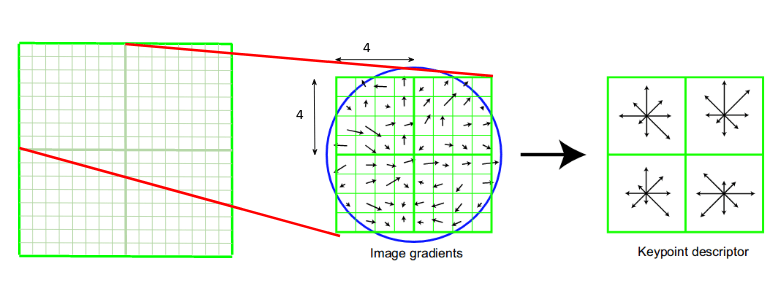
\includegraphics[width=0.4\linewidth]{image-gradients.png}
		\caption{\label{fig:image-gradients} SIFT's keypoint descriptor}
	\end{figure*}
	
	One of the 16 historgrams may look like this:
	
	\begin{figure*}
		\centering
		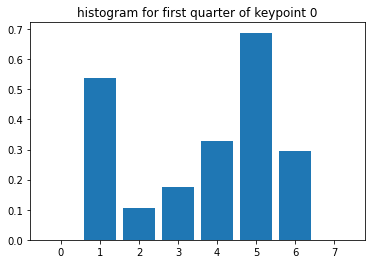
\includegraphics[width=0.4\linewidth]{8histogram.png}
		\caption{\label{fig:8histogram} One of the 16 8-bin orientation histograms in a keypoint's descriptor}
	\end{figure*}	
	
	\subsection{Keypoint Matching}
	Since we do not know exactly the format of the returned descriptor vectors returned by OpenCV built-in SIFT $detectAndCompute()$ method, it is safer to also implement our version keypoint matching instead of using OpenCV's $BFMatcher$. The process is implemented in the $matchDescriptors$ function in the notebook. In selection sort fashion, the method searches for matches between each of the descriptors in first and second set using the sum of square difference. The best and second best differences are kept tracked and evaluated using ratio rule suggested in Lowe's paper \cite{Lowe:2004:DIF:993451.996342}.
	
	\section{Result}
	Our SIFT process is finalized in the $sift()$ function and tested on two images provided in the $data$ folder. The result is undesirable \ref{output}. This means that despite following the document, we may still have some errors an unoptimized part in the process, thus need many fixes.
	
	\begin{figure*}
		\centering
		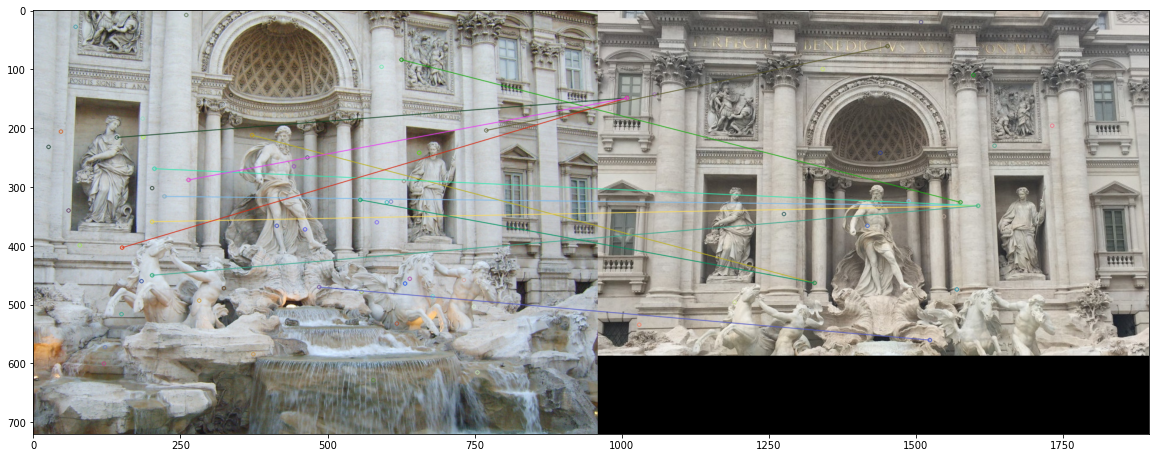
\includegraphics[width=0.8\linewidth]{output.png}
		\caption{\label{fig:output} The output of our version of SIFT}
	\end{figure*}
	
\end{multicols}

\newpage
\nocite{*}
\bibliographystyle{alpha}
\bibliography{bib}
		
\end{document}